\documentclass{beamer}
\usepackage[utf8]{inputenc}

\usetheme{Madrid}
\usecolortheme{default}
\usepackage{amsmath,amssymb,amsfonts,amsthm}
\usepackage{txfonts}
\usepackage{tkz-euclide}
\usepackage{listings}
\usepackage{adjustbox}
\usepackage{array}
\usepackage{tabularx}
\usepackage{gvv}
\usepackage{lmodern}
\usepackage{circuitikz}
\usepackage{tikz}
\usepackage{graphicx}

\setbeamertemplate{page number in head/foot}[totalframenumber]

\usepackage{tcolorbox}
\tcbuselibrary{minted,breakable,xparse,skins}



\definecolor{bg}{gray}{0.95}
\DeclareTCBListing{mintedbox}{O{}m!O{}}{%
  breakable=true,
  listing engine=minted,
  listing only,
  minted language=#2,
  minted style=default,
  minted options={%
    linenos,
    gobble=0,
    breaklines=true,
    breakafter=,,
    fontsize=\small,
    numbersep=8pt,
    #1},
  boxsep=0pt,
  left skip=0pt,
  right skip=0pt,
  left=25pt,
  right=0pt,
  top=3pt,
  bottom=3pt,
  arc=5pt,
  leftrule=0pt,
  rightrule=0pt,
  bottomrule=2pt,

  colback=bg,
  colframe=orange!70,
  enhanced,
  overlay={%
    \begin{tcbclipinterior}
    \fill[orange!20!white] (frame.south west) rectangle ([xshift=20pt]frame.north west);
    \end{tcbclipinterior}},
  #3,
}
\lstset{
    language=C,
    basicstyle=\ttfamily\small,
    keywordstyle=\color{blue},
    stringstyle=\color{orange},
    commentstyle=\color{green!60!black},
    numbers=left,
    numberstyle=\tiny\color{gray},
    breaklines=true,
    showstringspaces=false,
}
%------------------------------------------------------------
%This block of code defines the information to appear in the
%Title page
\title %optional
{2.7.3}
\date{\today}
%\subtitle{A short story}

\author % (optional)
{Shivam Sawarkar \\ AI25BTECH11031}



\begin{document}


\frame{\titlepage}
\begin{frame}{Question (2.7.3)}
If $\vec{a}$ and $\vec{b}$ are two vectors such that $\vec{a} = \hat{i} - \hat{j} + \hat{k}$, $\vec{b} = 2\hat{i} - \hat{j} - 3\hat{k}$, then find the vector $\vec{c}$, given that $\vec{a} \times \vec{c} = \vec{b}$, $\vec{a} \cdot \vec{c} = 4$.
\end{frame}

\begin{frame}{Solution}
\begin{align}
\vec{a} = \myvec{1 \\ -1 \\ 1} \quad 
\vec{b} = \myvec{2 \\ -1 \\ -3} \quad 
\vec{c} = \myvec{c_1 \\ c_2 \\ c_3}
\end{align}

\begin{align}
\vec{a}\times\vec{c} = \vec{b} \\ 
\myvec{-c_2 -c_3 \\ c_1-c_3 \\ c_1 + c_2}=\myvec{2 \\ -1 \\ -3}
\end{align}


\begin{align}
\implies 
\begin{cases}
-c_2-c_3 = 2,\\
c_1-c_3 = -1,\\
c_1+c_2 = -3.
\end{cases}
\end{align}
\end{frame}

\begin{frame}{Solution}
    From the second and third equations:
\begin{align}
c_1 = c_3 - 1, \qquad c_2 = -2 - c_3.
\end{align}

\begin{align}
\implies 
\vec{c} = \myvec{c_3-1 \\ -2-c_3 \\ c_3}, \quad c_3\in\mathbb{R}.
\end{align}
\end{frame}

\begin{frame}{Solution}
    Now apply the dot product condition:
\begin{align}
\vec{a}^T\vec{c} = \myvec{1 & -1 & 1}\myvec{c_3-1 \\ -2-c_3 \\ c_3} = 3c_3+1.
\end{align}

\begin{align}
3c_3+1=4 \quad \implies \quad c_3=1.
\end{align}

\begin{align}
\therefore \quad \vec{c} = \myvec{0 \\ -3 \\ 1}
\end{align}

\end{frame}

\begin{frame}{Plot}
    \begin{figure}
        \centering
        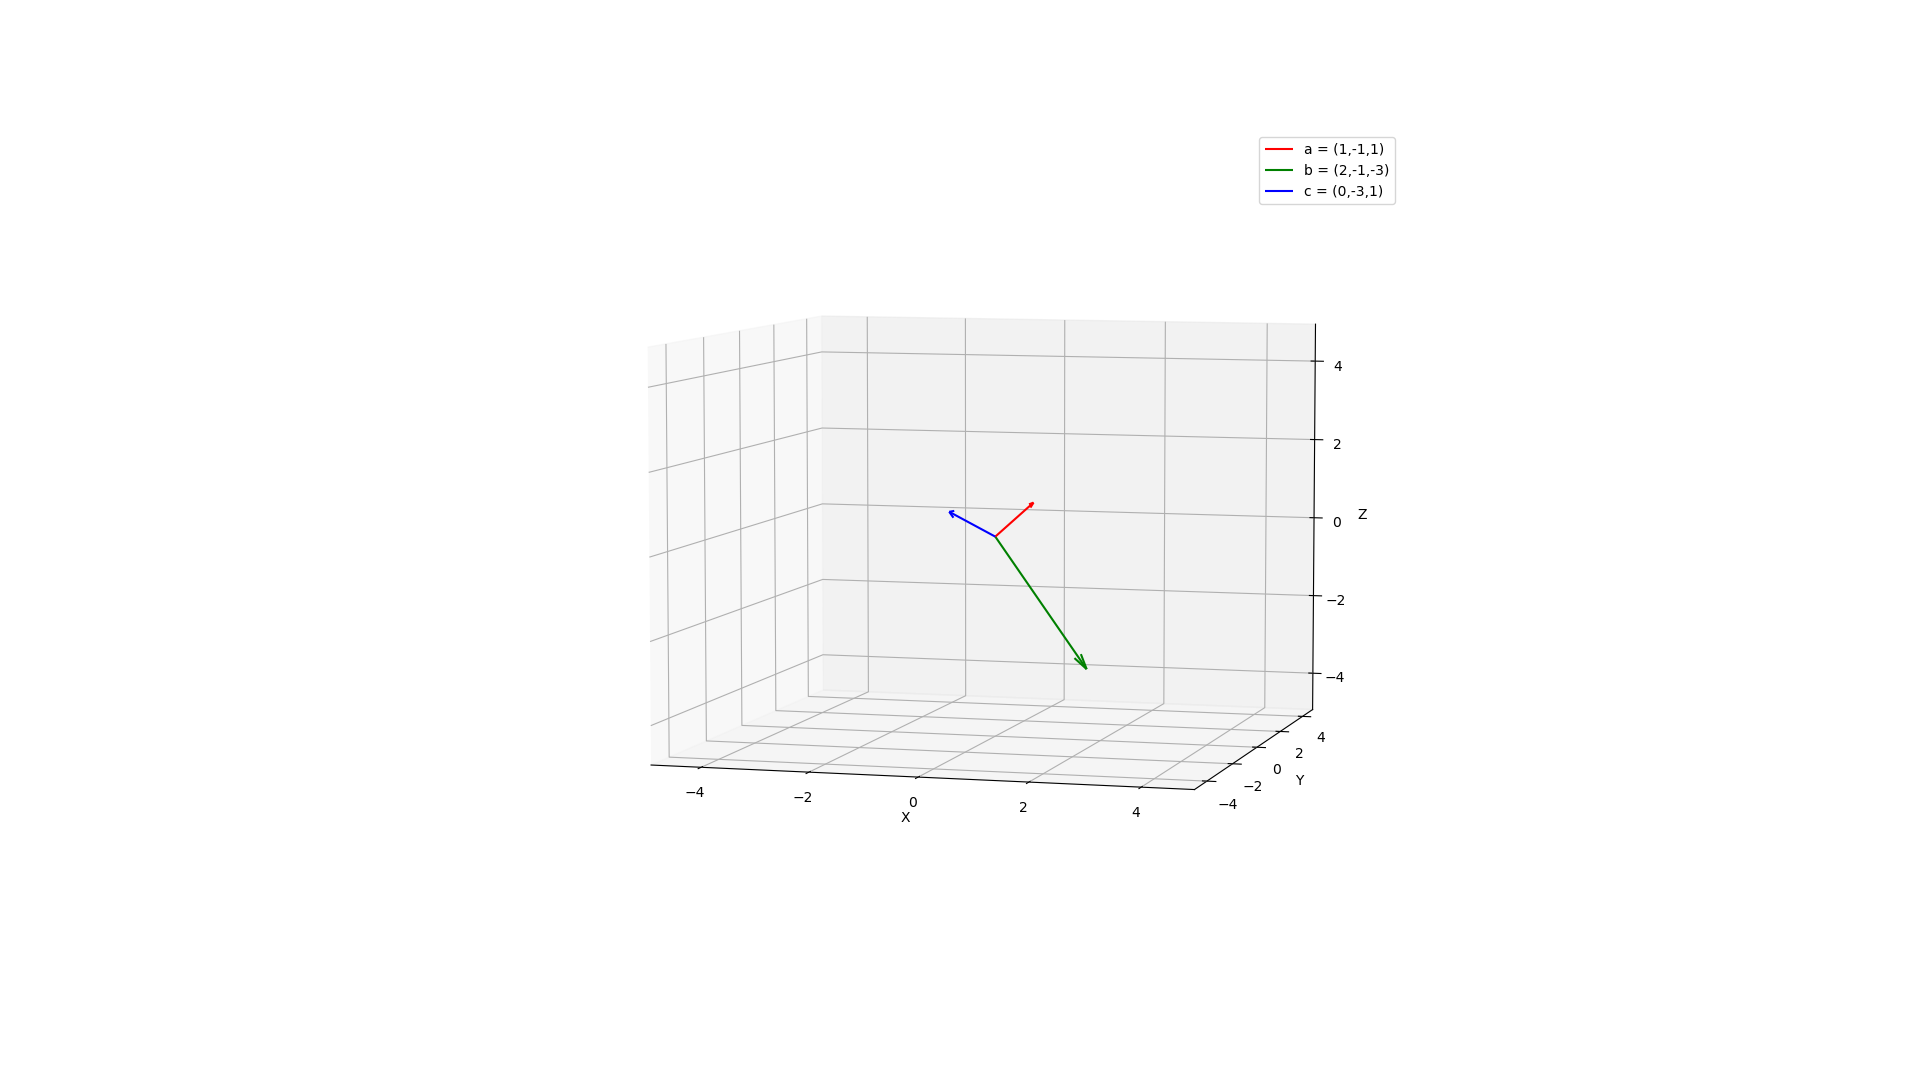
\includegraphics[width=1\columnwidth]{figs/plot4.png}
        \caption{}
        \label{fig:placeholder}
    \end{figure}
\end{frame}

\begin{frame}[fragile]{Python Code}
    \begin{verbatim}
import numpy as np

# Input vectors
a = np.array(list(map(int, input("Enter vector a (3 integers 
separated by space): ").split())))
b = np.array(list(map(int, input("Enter vector b (3 integers 
separated by space): ").split())))
dot_val = int(input("Enter value of a · c: "))

# Coefficient matrix (augmented form)
# Let c = (x,y,z)
# Equations:
#   a2*z - a3*y = b1
#   a3*x - a1*z = b2
#   a1*y - a2*x = b3
#   a1*x + a2*y + a3*z = dot_val
    \end{verbatim}
\end{frame}

\begin{frame}[fragile]{Python Code}
    \begin{verbatim}
A = np.array([
    [0, -a[2], a[1]],     # from a2*z - a3*y = b1
    [a[2], 0, -a[0]],     # from a3*x - a1*z = b2
    [-a[1], a[0], 0],     # from a1*y - a2*x = b3
    [a[0], a[1], a[2]]    # dot product
], dtype=float)

rhs = np.array([b[0], b[1], b[2], dot_val], dtype=float)

# Solve least squares (in case overdetermined)
c, residuals, rank, s = np.linalg.lstsq(A, rhs, rcond=None)

print("Vector c =", np.round(c, 4))
    \end{verbatim}
\end{frame}




\end{document}